\documentclass{article}
\usepackage[a4paper]{geometry}
\usepackage[utf8]{inputenc}
\usepackage{url}
\usepackage{hyperref}
\usepackage{multicol}
\usepackage{graphicx}
\usepackage{float}
\usepackage{mwe}
\usepackage{multirow}
\usepackage{listings}
\usepackage{csquotes}

\title{Atividade 1}
\author{Lucas Guesser Targino da Silva - RA: 203534\\
Lucas Pedroso Cantanhede - RA: 202058\\
Luiz Fernando Bueno Rosa - RA: 221197}

\newcommand{\Set}[1]{$\left\{#1\right\}$}
\newcommand{\Sum}[1]{\displaystyle\sum\limits_{#1}}

\begin{document}

\maketitle

\section{Modelo Matemático}

\subsection{Variáveis do Problema}
\label{constraint:exercise-variables}

\begin{itemize}
	\item $F$: Número de fábricas das companhias.
	\item $J$: Número de clientes das companhias.
	\item $L$: Número de máquinas das fábricas.
	\item $M$: Número de matérias-primas das fábricas.
	\item $P$: Número de tipos de produtos produzidos pelas fábricas.
	\item $D_{j,p}$: Demanda do cliente $j$, em toneladas, do produto $p$.
	\item $r_{m,p,l}$: Quantidade de matéria-prima $m$, em toneladas, necessária para produzir uma tonelada do produto $p$ na máquina $l$.
	\item $R_{m, f}$: Quantidade de matéria-prima $m$, em toneladas, disponível na fábrica $f$.
	\item $C_{l,f}$: Capacidade disponível de produção, em toneladas, da máquina $l$ na fábrica $f$.
	\item $p_{p,l,f}$: Custo de produção, por tonelada, do produto $p$ utilizando a máquina $l$ na fábrica $f$.
	\item $t_{p,f,j}$: Custo de transporte, por tonelada, do produto $p$ partindo da fábrica $f$ até o cliente $j$.
\end{itemize}

\subsection{Variáveis de Decisão}

\begin{itemize}
	\item $x_{p,l,f}$: quantidade, em toneladas, do produto $p$ produzida na máquina $l$ da fábrica $f$.
	\item $y_{p,f,j}$: quantidade, em toneladas, do produto $p$ transportada da fábrica $f$ para o cliente $j$.
\end{itemize}


\subsection{Objetivo}

Minimizar:
\begin{equation}
    \label{objective}
 	\Sum{p}\Sum{l}\Sum{f} p_{p,l,f} \  x_{p,l,f}
	+
	\Sum{p}\Sum{f}\Sum{j} t_{p,f,j} \  y_{p,f,j}
\end{equation}

Sujeito a:
\begin{equation}
	\label{constraint:demand}
	D_{j,p} = \Sum{f} y_{p,f,j}
	\quad \forall p \ \forall j
\end{equation}

\begin{equation}
	\label{constraint:resources}
	R_{m,f} \geq \Sum{p} \Sum{l} r_{m,p,l} \ x_{p,l,f}
	\quad \forall m \ \forall f
--\end{equation}

\begin{equation}
	\label{constraint:production-capacity}
	C_{l,f} \geq \Sum{p} x_{p,l,f}
	\quad \forall l \ \forall f
\end{equation}

\begin{equation}
	\label{constraint:compatibility}
	\Sum{l} x_{p,l,f} = \Sum{j} y_{p,f,j}
	\quad \forall p \ \forall f
\end{equation}

\begin{equation}
	\label{constraint:non-negativity}
	x_{p,l,f}, y_{p,f,j} \geq 0
	\quad \forall p \ \forall l \ \forall f \ \forall j
\end{equation}

A notação $\forall i$ acima (podendo $i$ ser $p, l, f, m, j$) significa que a restrição se aplica a todos os valores do domínio discreto de $i$. Por exemplo, se o domínio de $f$ for \Set{1, 2, 3}, então a condição se aplica para $f=1$, $f=2$ e $f=3$. Esse modelo ainda não usa \cite{bib:gurobi}.

Iremos explicar, brevemente, o que cada restrição significa:

\begin{enumerate}
    \item A função objetivo \ref{objective} é calculada como sendo a soma do custo de produção (somatório à esquerda) e o custo de transporte (somatório à direita). O custo de produção é calculado como uma soma variando para cada produto $p$, máquina $l$ e fábrica $f$ da quantidade produzida, em toneladas, vezes o custo por tonelada $p_{p,l,f}$. O custo de transporte é calculado como uma soma variando para cada produto $p$, fábrica $f$ e cliente $j$ da quantidade transportada, em toneladas, vezes o custo de transporte $t_{p,f,j}$. Tendo em vista que queremos o menor custo possível, temos que o objetivo é minimizar o máximo possivel o resultado dessa função.

    \item A restrição \ref{constraint:demand} é a restrição da demanda onde restringimos que a demanda solicitada ($D_{j,p}$) por qualquer cliente $j$ de um produto $p$, deve ser igual a somatória da quantidade de $p$ de produtos produzidos e transportados para esse cliente $j$ em todas as fábricas.

    \item A restrição \ref{constraint:resources} é a restrição de produção de um produto $p$ na fábrica $f$ onde $r_{m, p, l}$ é a quantidade em toneladas do material $m$ necessário para produzir uma tonelada de $p$ na máquina $l$ e $R_{m, f}$ é a quantidade de $m$ na fábrica $f$.

    \item A restrição \ref{constraint:production-capacity} é a restrição da capacidade produtiva restringimos que a capacidade disponível, em toneladas, de produção de qualquer máquina $l$ em uma fábrica $f$ deve igual ou superior a somatória da quantidade, em toneladas, produzida de produtos $p$ por essa mesma máquina $l$ na fábrica $f$.

    \item A restrição \ref{constraint:compatibility} é a restrição de compatibilidade entre o que foi produzido e que foi transportado. Nela consideramos que existe uma igualdade da somatória da quantidade, em toneladas, produzida em todas as fábricas de qualquer produto $p$ em determinada máquina $m$ com a somatória da quantidade, em toneladas, transportada para todos os clientes desse mesmo produto $p$ produzido pela máquina $m$.

    \item A restrição \ref{constraint:non-negativity} é a restrição de não-negatividade, considerando que nem $x_{p,l,f}$ nem $y_{p,f,j}$ podem ser negativos independentes dos valores de $p$, $l$, $f$ e $j$.
\end{enumerate}


\subsection{Geração das instâncias}

Conforme solicitado no enunciado, geramos 10 instâncias aleatórias variando a quantidade de clientes $|J| = {100, 200, 300, 400, 500, 600, 700, 800, 900, 1000}$ e os demais parâmetros do enunciado, apresentados em \ref{constraint:exercise-variables}, de maneira aleatória e uniforme seguindo as restrições dos coeficientes abaixo:

\begin{itemize}
	\item $|F| \in [|J|,2|J|]$
	\item $|L| \in [5,10]$
	\item $|M| \in [5,10]$
	\item $|P| \in [5,10]$
	\item $D_{j,p} \in [10,20]$
	\item $r_{m,p,l} \in [1,5]$
	\item $R_{m, f} \in [800,1000]$
	\item $C_{l,f} \in [80,100]$
	\item $p_{p,l,f} \in [10,100]$
	\item $t_{p,f,j} \in [10,20]$
\end{itemize}

O módulo de geração de números aleatórios empregado foi \verb|numpy.random| da biblioteca numpy \cite{bib:numpy}. Utilizou-se a semente de números aleatórios \verb|17558175| para gerar, de forma que tenha-se as mesmas instâncias de problemas em diferentes execuções do código.

\subsection{Configuração da Máquina}

O problema foi executado num ideapad S145 81S90005BR: Lenovo IdeaPad S145 Notebook Intel Core i5-8265U (6MB Cache, 1.6GHz), 8GB DDR4-SDRAM, 460 GB SSD, Intel UHD Graphics 620.

O sistema operacional foi o Fedora 35 executando o Python 3.7.12 e Gurobi Optimizer v9.5.1rc2.

\subsection{Resultados}

\begin{center}
\begin{tabular}{||c c c c c||}
\hline
\label{table:result}
  Instância(J) & Qtde. de variáveis & Qtde. de restrições & Custo da Solução & Tempo de execução(s) \\
 \hline\hline
 100 & 100320 & 3422 & 253714.11620693645 & 3.263497  \\
 \hline
 200 & 668817 & 9698 & 567490.8153045126 & 18.304874\\
 \hline
 300 & 1441176 & 18141 & 744867.1786728669 & 60.564301 \\
 \hline
 400 & 1909440 & 16070 & 994991.7809754083 & 97.239349 \\
 \hline
 500 & 1771000 & 13700 & 790455.3006384401 & 50.536251 \\
 \hline
 600 & 3981420 & 20454 & 1929256.3805292659 & 222.136828 \\
  \hline
\end{tabular}
\end{center}

Devido a limitações de recursos computacionais (memória), não foi possível rodar instâncias geradas com $J \geq 700$. Porém, os dados coletados já são suficientes para o propósito de aprendizado do trabalho.

\subsection{Análise}

\subsubsection{Tempo de execução}

A partir dos dados da tabela anterior, utilizamos uma regressão linear para estudar o crescimento do tempo de execução. A suspeita inicial é que encontraríamos um crescimento polinomial, isto é, que cresce em $O(n^k)$.

Mas, primeiramente, observe na tabela \ref{table:result} de resultados acima a instância $J=500$. É o primeiro caso que possa apontar um comportamento não-linear da nossa função, então um experimento interessante seria plotar os nossos tempos de execução ora levando em conta $J=500$ ora não e tentar estimar visualmente o crescimento da nossa função.

Os gráficos a seguir são uma plotagem do tempo de execução em relação ao número de clientes $|J|$ juntamente com uma estimativa linear desses dados, gerada a partir do algoritmo de regressão linear.

\begin{figure}[!ht]
\label{figura:1}
\begin{multicols}{2}

    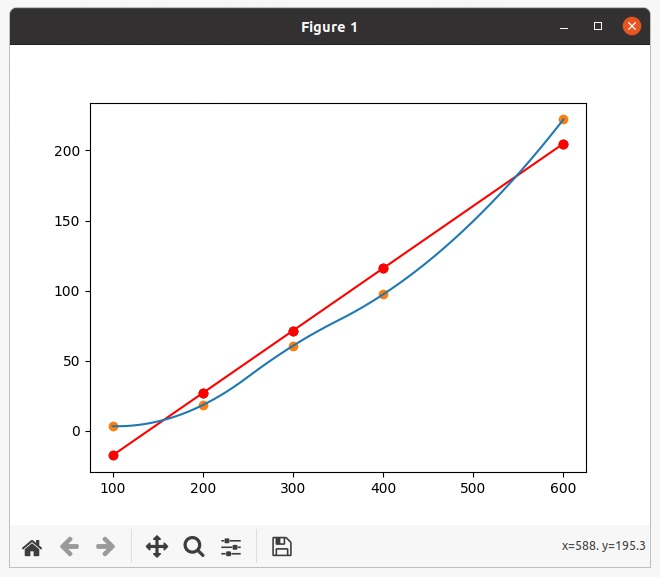
\includegraphics[width=\linewidth]{execucao_sem_J=500.jpeg}\par
    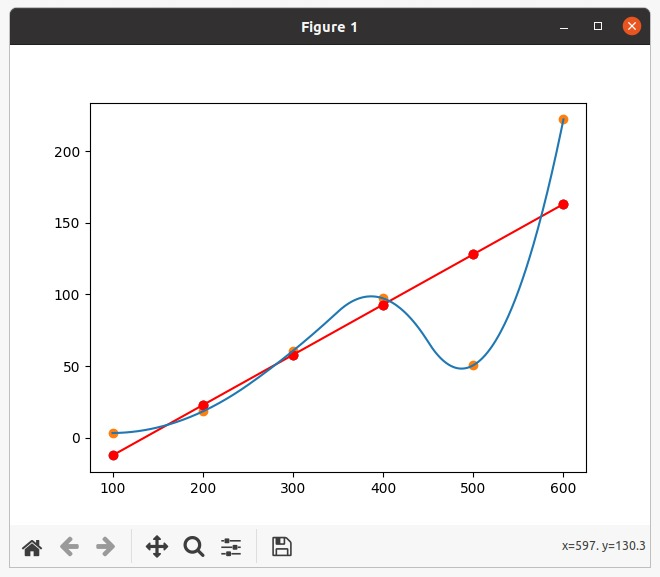
\includegraphics[width=\linewidth]{execucao_com_J=500.jpeg}\par

\end{multicols}
\caption{O gráfico da esquerda apresenta os dados sem o ponto $J=500$ enquanto o da direita inclui esse ponto. Perceba que, sem o outlier, identificamos uma tendência linear.}
\end{figure}

No entanto, seriam necessários mais dados para podermos ter uma acurácia melhor de como o tempo de execução se comporta, pois se isolarmos os pontos $J=400$, $J=500$ e $J=600$, percebemos uma tendência exponencial no gráfico.

Mas é certo afirmar que a tendência é linear na maior parte dos amostras recolhidas, o que vai de acordo com as nossas suspeitas.

\subsubsection{Minimização de custos}

Podemos realizar as mesmas análises em relação à minimização da função objetivo. Hipotetizamos que, como a função objetivo é linear, então a sua minimização deve ser proporcional ao aumento da demanda(número dos clientes).

\begin{figure*}[!ht]
\begin{multicols}{2}

    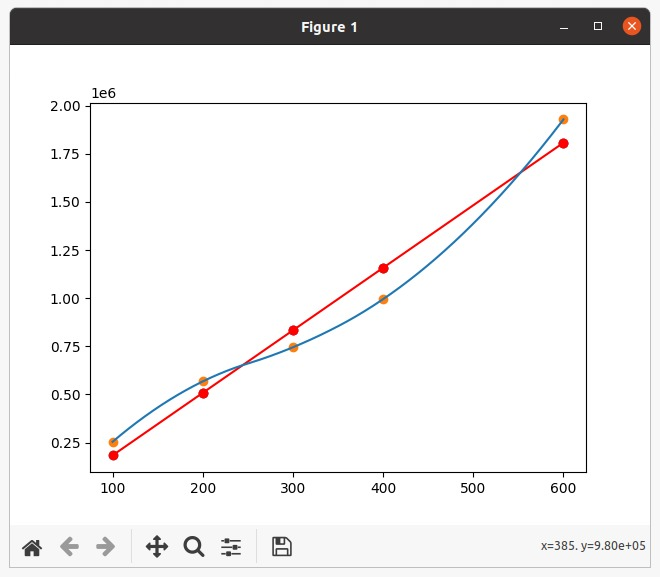
\includegraphics[width=\linewidth]{minimizacao_sem_J=500.jpeg}\par
    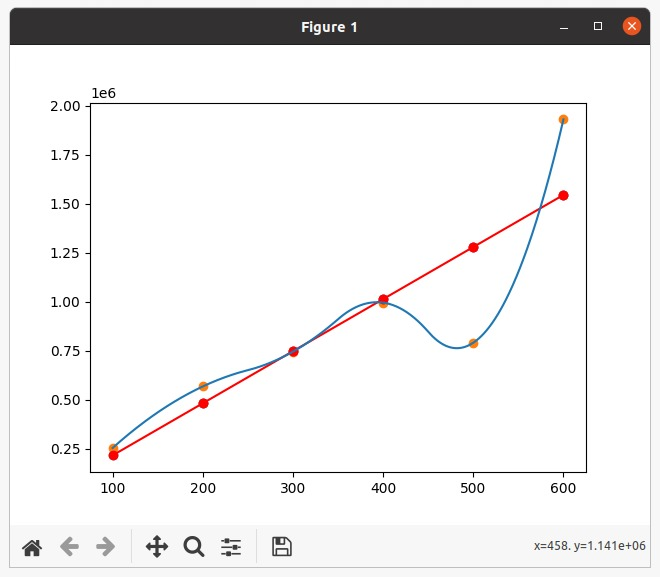
\includegraphics[width=\linewidth]{minimizacao_com_J=500.jpeg}\par

\end{multicols}
\caption{O gráfico da esquerda apresenta os dados sem o ponto $J=500$ enquanto o da direita inclui esse ponto. Perceba que, sem o outlier, identificamos, novamente, uma tendência linear.}
\end{figure*}

Conseguimos averiguar pelos dois gráficos anteriores que o crescimento da minimização da função objetivo possui a mesma tendência que o crescimento do tempo de execução, o que confirma nossa hipótese.

\section{Referências}

\bibliographystyle{unsrt}
\bibliography{bibliography}

\end{document}
